\documentclass[10pt,a4paper]{article}
\usepackage[latin1]{inputenc}
\usepackage{amsmath}
\usepackage{amsfonts}
\usepackage{amssymb}
\usepackage{graphicx}
\usepackage[left=3.00cm, right=3.00cm, top=3.00cm, bottom=3.00cm]{geometry}
\begin{document}
	\paragraph{Candidato}Alex Foglia
	\paragraph{Titolo}Analisi di un sottosistema di posizionamento ferrotramviario
	\paragraph{Relatore}Andrea Bondavalli
	\paragraph{Riassunto}I sistemi di posizionamento ferroviari e ferrotramviari ad oggi impiegati, fanno un largo uso di apparati installati a terra e segnali provenienti dalla linea. La loro realizzazione ha pertanto un costo e un impatto ambientale non trascurabili. Per questo motivo, \`e necessario pianificare una migrazione verso di sistemi di posizionamento autonomi, in accordo alle normative operazionali europee in ambito ferroviario e ferrotramviario definite dallo standard \texttt{ERTMS/ETCS}.\\*
	Un sistema di posizionamento ferroviario, o ferrotramviario, \`e autonomo quando non fa alcun uso di apparati installati a terra.\\*
	In questa Tesi si mostrano, e discutono, i risultati sperimentali ottenuti attraverso un' attivit\`a di \emph{fault injection} condotta su un sottosistema di posizionamento ferrotramviario autonomo.\\*
	Il sistema \emph{target} dell'analisi basa il suo funzionamento sull'utilizzo di un insieme di sensori installati a bordo treno, le cui misure campionate vengono processate da un algoritmo noto come \emph{Sensor Fusion Algorithm} (SFA).\\*
	SFA \`e un algoritmo che integra le misure fornite da un insieme di sensori al fine di attutirne il rumore di misura. L'output prodotto da SFA \`e una misura pi\`u sicura e affidabile di quella che si otterrebbe considerando i sensori singolarmente. In questo contesto, la misura che si intende fornire attraverso l'uso di SFA \`e la posizione del treno.\\*
	Per le sue caratteristiche architetturali, \`e possibile classificare il sistema come un \emph{Cyber Physical Systems of Systems} (CPSoS), mentre il particolare dominio applicativo colloca il sistema nell'area \emph{safety-critical}.\\*
	La Tesi passa in rassegna lo stato dell'arte circa la valutazione della \emph{dependability} di un sistema e le tradizionali tecniche di posizionamento ferroviario. Segue poi una descrizione del sistema, del suo contesto operativo nominale e degli standard che lo regolamentano. Si descrive l'ambiente in cui il sistema verr\`a analizzato, e infine si discutono i risultati dell'analisi condotta.\\*
	Attraverso l'attivit\`a di \emph{fault injection} \`e stato principalmente osservato che il sistema \`e in grado di tollerare bene guasti al sistema di comunicazione verso i sensori, a condizione che rimanga funzionante almeno un canale: quello verso il \emph{sensore inerziale}.\\*
	Il sistema sembra inoltre capace di individuare, e correggere di conseguenza, i messaggi ricevuti che hanno un' elevata probabilit\`a di contenere un dato sbagliato.
	\newpage
	\begin{figure}
		\centering
		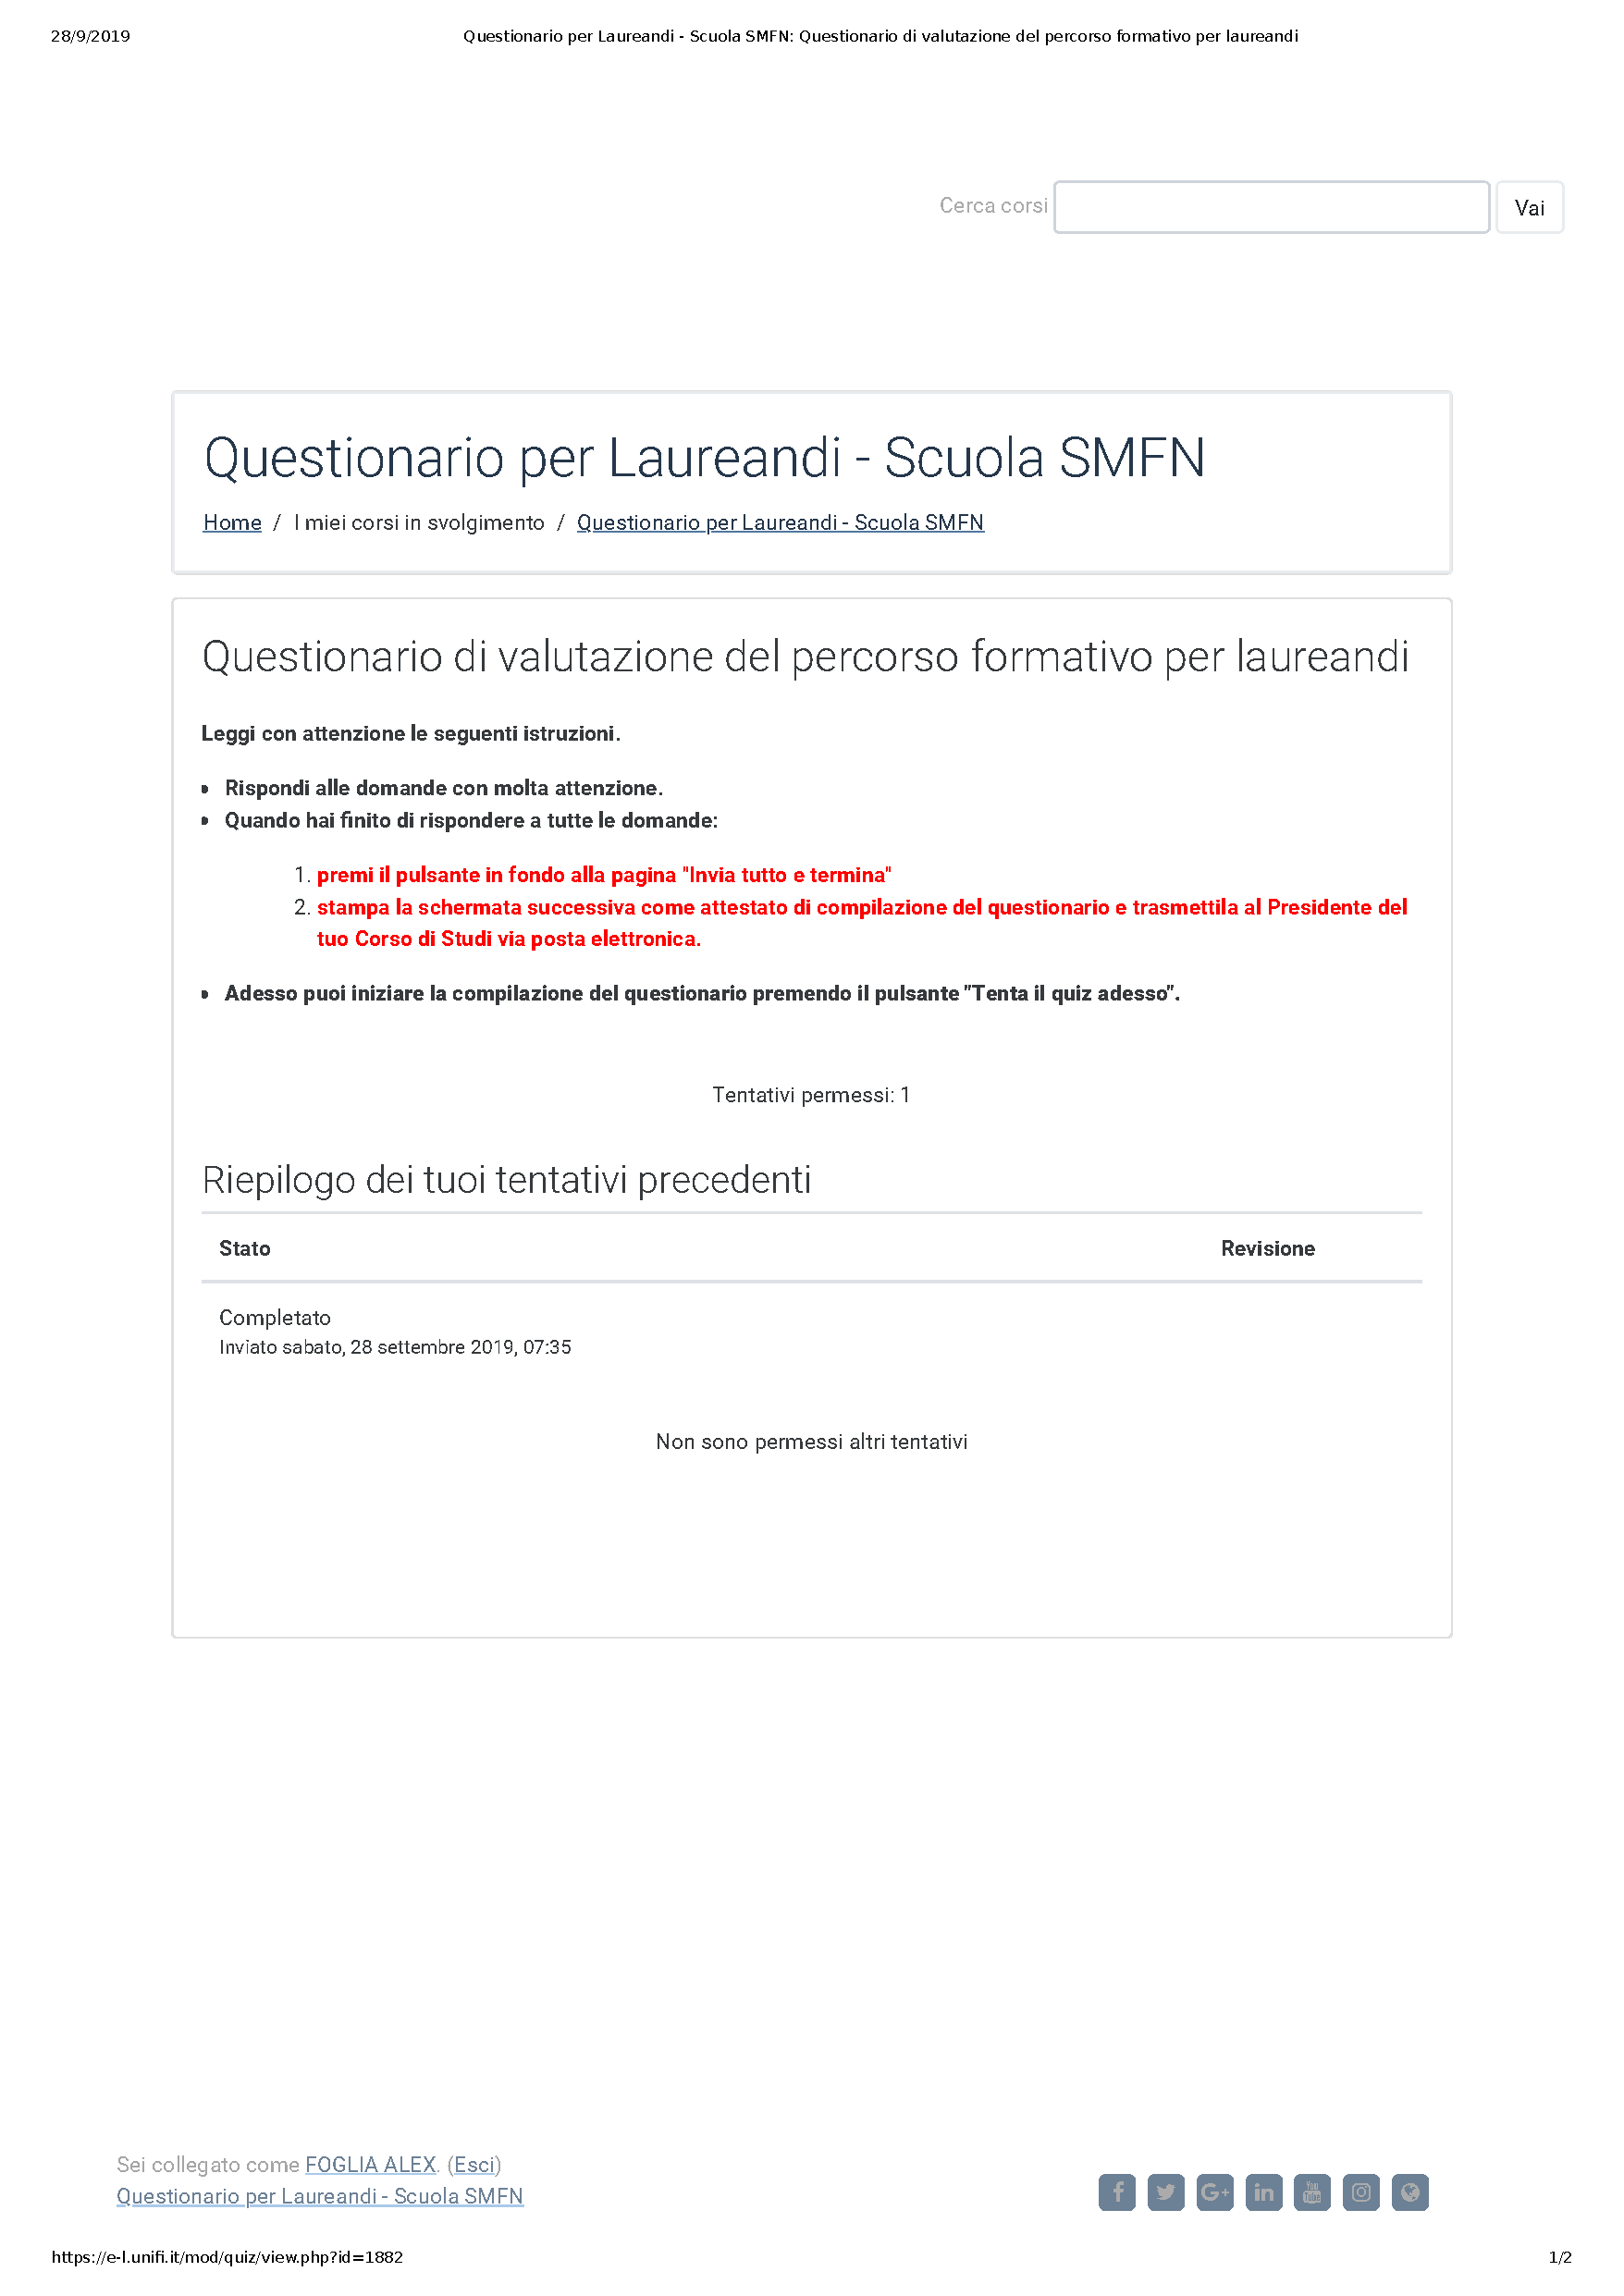
\includegraphics[width=\linewidth]{questionario}
		\label{fig:questionario}
	\end{figure}
	
	
\end{document}